% Capitulo 2

\chapter{Redes federadas eventualmente conectadas}
\label{Capitulo2}
\lhead{Cap\'itulo 2. \emph{Redes federadas eventualmente conectadas}}


Com rede federada pode se entender um universo muito amplo de
situações. Neste trabalho se considera principalmente uma rede
federada que tenha as seguintes caraterísticas:

\begin{itemize}
  \item administração descentralizada
  \item acesso a gestão logica (e física) da rede
  \item conhecimentos técnicos locais das tecnologias usadas na rede
  \item serviços internos a rede federada
  \item interações entre redes locais inteligentes
\end{itemize} 

Uma rede federada, então, entendida como um conjunto de soluções
tecnicamente viáveis e adaptáveis a usos, praticas e contextos
diferentes, que permita uma gestão flexível da rede, com sub-redes
heterogêneas, aproveitando diversas tecnologias, como por exemplo P2P
onde necessário. Uma rede federada se adapta particularmente num
contexto onde já existe uma estrutura organizacional que pode se
espelhar na estrutura da rede e que pode acompanhar sua gestão. 

\section{Redes federadas eventualmente conectadas}
A introdução sobre o contexto sugere o âmbito de estudo mas necessita
uma restrição maior. Para ``redes federadas eventualmente conectadas''
consideramos, uma rede federada baseada em conexões não sempre
disponíveis, como as conexões por satélite, com a exigência de manter
os serviços federados ativos, mesmo em ausência de comunicação. Os
serviços federados são, ainda, otimizados para a resiliência do
sistema e a redução do trafego de rede externo, através de estrategias
de replicação, sincronização e memorização dos dados na infraestrutura
logico/física local.

\section{A Rede Mocambos}   
\label{sec:RedeMocambos}

\begin{quote}
  ``\emph{É uma rede solidária de comunidades, no qual o objetivo
    principal é compartilhar idéias e oferecer apoio recíproco.}''
  \ldots ``\emph{A tecnologia é uma frente de trabalho da Rede
    Mocambos, sendo ao mesmo tempo idéia e meio para transferir
    idéias.}'' \citep{RMSobre}.
\end{quote}

A Rede Mocambos (RM), atualmente envolve diretamente mais de duzentas
comunidades quilombolas, coletivos, aldeias indígenas, pontos de
cultura e terreiros (ver figura \ref{fig:MappaRedeMocambos}). Existem
dois termos de cooperação\footnote{Os termos de cooperação foram
  assinados, como Rede Mocambos, mas formalmente pela Casa de Cultura
  Tainã.} entre Rede Mocambos e o Ministério das Comunicações,
precisamente com os programas GESAC e Telecentros.BR.

\begin{figure}[htbp]
  \centering
  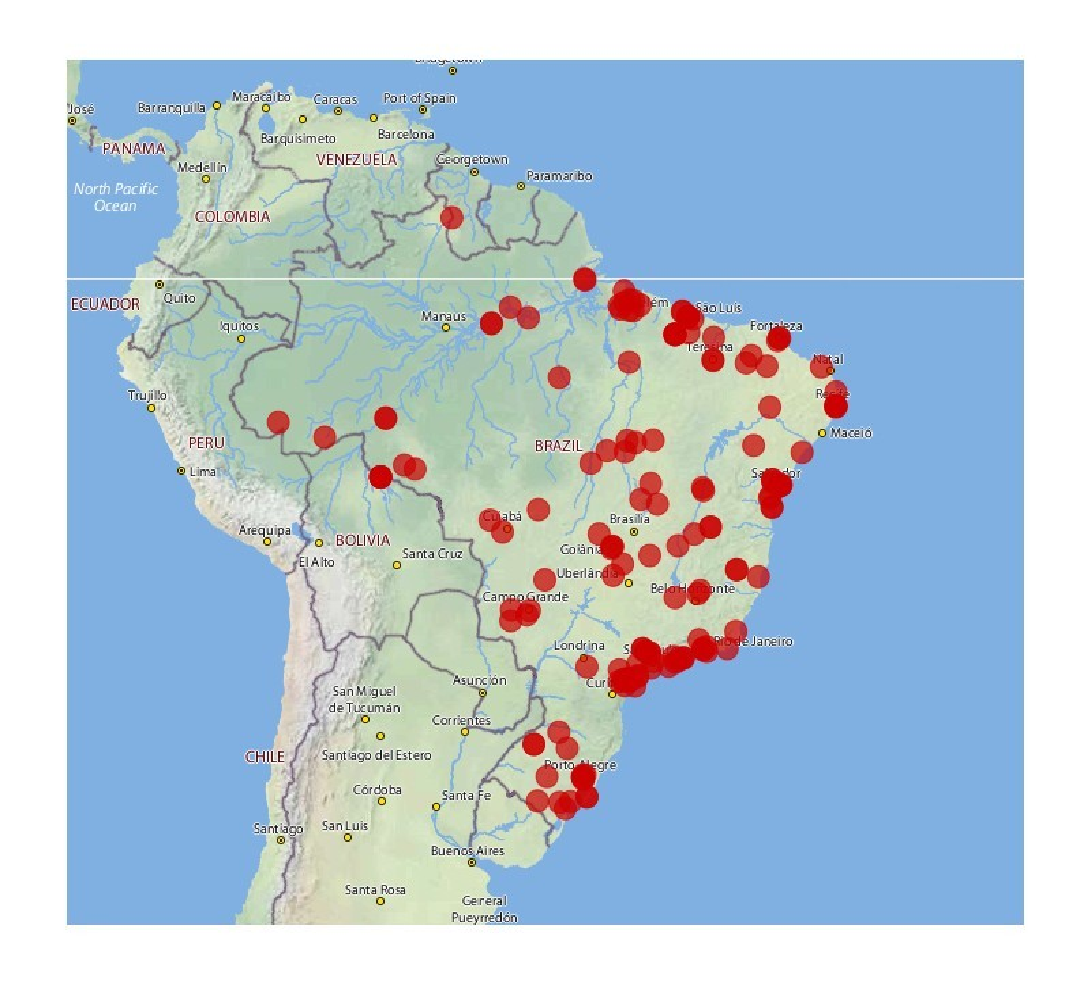
\includegraphics[width=\textwidth]{./Figure/MappaRedeMocambos.pdf}
  \rule{35em}{0.5pt}
  \caption[Mapa das comunidades da Rede Mocambos, retirado desde
  \url{http://mapa.mocambos.net}]{Mapa das comunidades da Rede Mocambos, retirado desde
  \url{http://mapa.mocambos.net}}
  \label{fig:MappaRedeMocambos}
\end{figure}

O GESAC garante conectividade por satélite a todas as comunidades, com
banda limitada devido a tipologia de tecnologia, que devido as
distancias representa a única alternativa, pelo menos no curto e médio
prazo. Através do programa Telecentros.BR estão sendo instalados
telecentros, salas equipadas com computadores para acesso publico, e
garantidas bolsas para monitores, para a gestão desses espaços. É
exatamente em contextos tão específicos que nasce a necessidade de
adaptar a tecnologia as exigências locais, também pelas limitações
técnicas impostas. A escassez de banda leva a reconsiderar a rede não
somente como o meio de conexão para os grandes \emph{data centers}. A
rede pode, e neste caso deve, ser estruturada no território com
logicas de desenvolvimento e gestão local determinadas pelas
comunidades. Neste sentido é fundamental a formação e o acesso as
tecnologias. A Casa de Cultura Tainã, núcleo fundador da Rede
Mocambos, e entre as primeira realidades populares que perceberam a
necessidade do Software Livre, como expressão de liberdade de poder
criar as próprias ferramentas tecnológicas digitais. A exclusão
digital não diz respeito somente ao acesso ao mundo digital mas também
da impossibilidade de participar a sua criação e desenvolvimento.



% \begin{figure}[htbp]
%   \centering
%   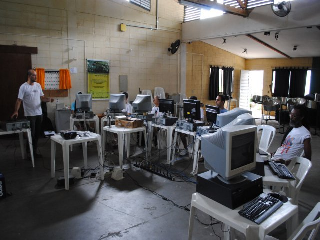
\includegraphics[width=\textwidth]{./Figure/taina_oficina.pdf}
%   \rule{35em}{0.5pt}
%   \caption[Laboratorio di grafica 3D con Blender alla \emph{Casa de
%     Cultura Tainã}]{Laboratorio di grafica 3D con Blender alla
%     \emph{Casa de Cultura Tainã}}
%   \label{fig:oficinaBlender}
% \end{figure}

\begin{figure}[htbp]
  \centering
  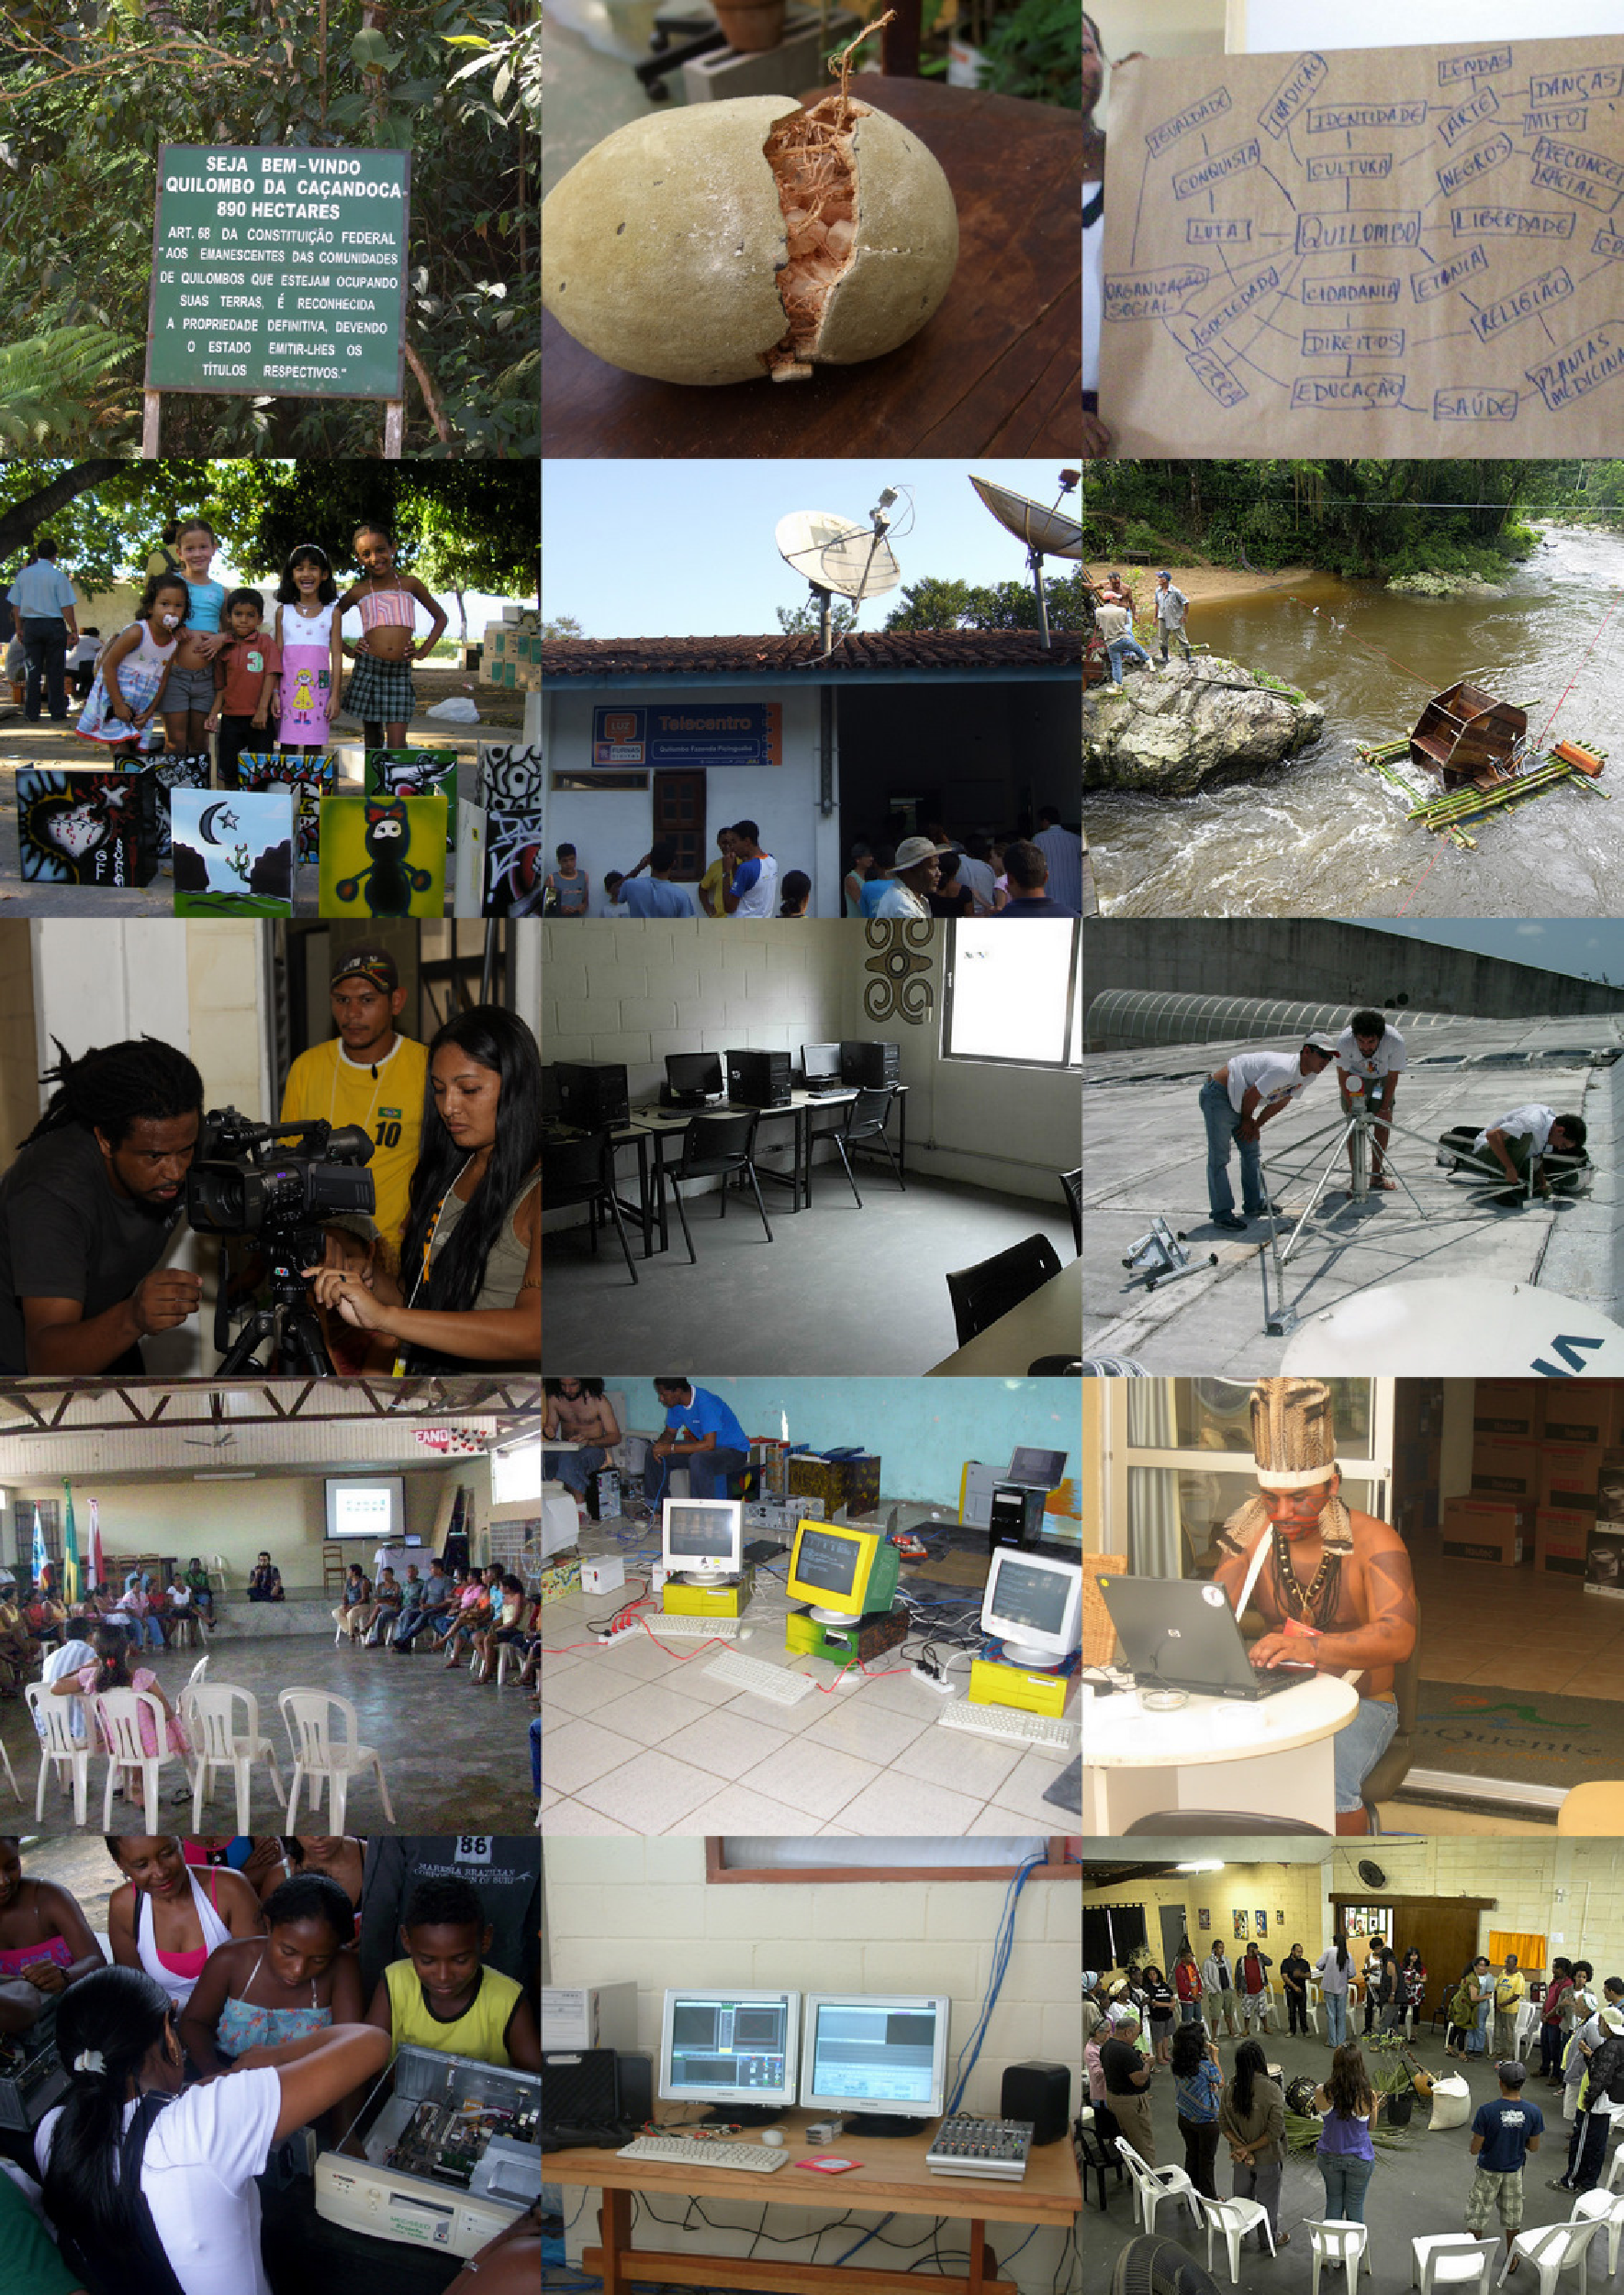
\includegraphics[width=\textwidth]{./Figure/FotoTesi.pdf}
  \rule{35em}{0.5pt}
  \caption[Fotos da Rede Mocambos]{Fotos da Rede Mocambos}
  \label{fig:FotoRM}
\end{figure}

Para a RM é importante, por vários aspectos, poder construir e gerir
os meios de comunicação e adaptá-los a seu contexto. No Brasil são
muitas as comunidades indígenas, quilombolas e tradicionais que
conhecem bem as potencialidades das tecnologias digitais e estão, cada
vez mais, dominando-as. Isso não teria sido possível sem a existência
e ampla difusão de Software Livre. Tecnologias digitais sob forma de
produtos comerciais seriam o enésimo passo para uma dependência
econômica e cultural. Esta consciência esta atras de escolhas bem
ponderadas. Alguns anos atras, em Brasília, numa reunião
do programa Luz Para Todos, programa federal para levar a eletricidade
a população da área rural, um cacique disse que, mesmo querendo a
energia elétrica, este devia ser limitada aos espaços comunitários e
não devia ser ligada nas casas. Não é difícil entender o porque de tal
condição. Além dos aspectos culturais, ter um contador e uma conta
para cada casa significaria introduzir custos em dinheiro, que não são
compatíveis com a economia deles. 

\section{Tecnologias}
Antes de mergulhar nos requisitos específicos, e nas escolhas feitas,
pode ser útil uma breve descrição das ferramentas tecnológicas que de
várias formas foram usadas para estruturar o protótipo, para a Rede
Mocambos, de rede federada eventualmente conectada, em particular para
os seus serviços de base, como a identificação, autenticação e
comunicação. 

\subsection{LDAP}
\emph{Lightweight Directory Access Protocol (LDAP)}\footnote{Protocolo
  Leve de Acesso a Diretório.} é um conjunto de protocolos abertos
para acessar as informações mantidas centralmente através uma
rede. LDAP organiza as informações através de uma hierarquia a arvore
chamada \emph{Directory Information Tree (DIT)}\footnote{Arvore do
  diretório de informações}. LDAP é um sistema cliente/servidor. O
servidor pode usar uma variedade de banco de dados para armazenar um
DIT, normalmente otimizados para operações de leitura. Quando uma
aplicação cliente se conecta a um servidor LDAP, pode ou consultar o
diretório ou tentar de alterá-lo. No caso de uma consulta, o servidor
pode responder de maneira local, ou pode encaminhar o pedido para um
servidor LDAP em condição de responder. Se a aplicação cliente esta
tentando modificar informações do diretório LDAP, o servidor verifica
se o usuário possui permissão de efetuar a mudança, para em seguida
adicionar e atualizar as informações. LDAP suporta a delegação de
parte do DIT para servidores específicos, a replicação só em leitura e
a replicação em leitura/escritura (chamada \emph{multi-master}). LDAP
é um protocolo solido, muito comum e suportado, e desde muito tempo è
o padrão de facto para gerir base de dados de usuários. OpenLDAP é uma
implementação aberta e livre do protocolo LDAP, que inclui cliente,
servidor e uma serie de ferramentas para facilitar a administração.
  
\subsection{XMPP}
Extensible Messaging and Presence Protocol (XMPP)\footnote{Protocolo
  extensível para mensagens e presencia.} é um conjunto de protocolos
abertos para as mensagens e a presença em rede baseado no XML. XMPP é
um sistema cliente/servidor. As especificações para a comunicação
entre servidores permitem que os usuários de um servidor interajam de
maneira transparente com usuários de outros servidor federados. A
\emph{XMPP Standard Foundation (XSF)} coordena o desenvolvimento das
extensões do padrão por meio das \emph{XMPP Extensions Protocols
  (XEPs)}, que até hoje são já 311. XMPP e as XEPs constituem um
ambiente flexível e completo para o desenvolvimento de serviços
federados. Estes protocolos são já usáveis graças as muitas
implementações de servidores, clientes e bibliotecas livres. A
história do XMPP, uma vez conhecido como Jabber, também é
interessante. Jabber foi inicialmente desenvolvido por Jeremie Miller
na sua fazenda no Iowa. É um exemplo concreto de como a pesquisa e o
desenvolvimento de tecnologias da comunicação, fora de ambientes
acadêmicos e empresariais, além de possível pode ser
revolucionaria. De facto, hoje, XMPP é a tecnologia mais usada para
mensagens instantâneas também pelo grandes atores da \emph{new economy}.

Para as necessidade específicas de uma rede é possível então estender
e customizar as funcionalidades do próprio servidor XMPP a ao mesmo
tempo usufruir dos serviços base, mensagens e presencia, implementados
pelos servidores já existentes na rede. 

\subsection{OpenID}
OpenID é um sistema de identificação descentralizada no qual a própria
identidade é uma URL que pode ser verificada por qualquer serviço que
suporte o protocolo. É um protocolo aberto e são disponíveis várias
implementações livres. Além disso o protocolo foi adotada pelos
principais provedores de serviços web. Com OpenID é possível usar a
mesma identidade em mais serviços e é uma ótima base para um sistema
\emph{Single Sign On (SSO)}. O protocolo utiliza HTTP e \emph{Cookies}
para manter uma sessão ativa. No primeiro tentativo de autenticação em
um serviço compatível com OpenID, o usuário é redirecionado para o
próprio provedor OpenID para efetuar o acesso e confirmar a
autorização a proceder com o serviço inicial. Por toda a durada da
sessão, é possível acessar serviços OpenID sem reinserir as
credenciais. 

\begin{figure}[htbp]
  \centering
  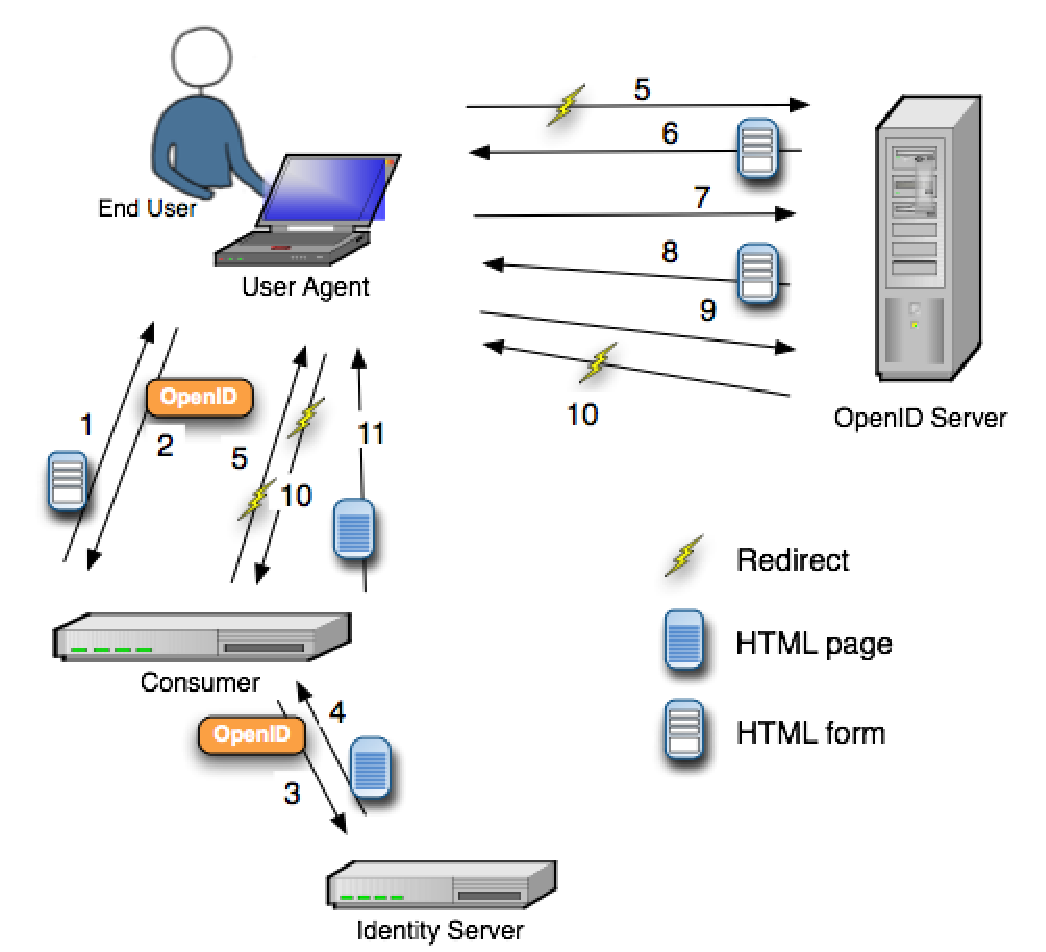
\includegraphics[width=0.6\textwidth]{./Figure/OpenID_Scenario.pdf}
  \rule{35em}{0.5pt}
  \caption[Diagrama de autenticação de OpenID]{Diagrama de autenticação de OpenID}
  \label{fig:OpenID}
\end{figure}

\subsection{OAuth}
OAuth é um protocolo aberto para autorização de serviços através
API. Por exemplo, permite para um usuário autorizar o acesso a
informações específicas armazenadas num site, chamado \emph{service
  provider}, para outro site, chamado \emph{consumer}, sem necessidade
de compartilhar a sua identidade. É uma maneira de publicar e
interagir com dados protegidos. Existem muitos outros protocolos e API
parecidos como Google AuthSub, AOL OpenAuth, Yahoo
BBAuth, Upcoming API, Flickr API, Amazon Web Services e cada um
fornece maneiras proprietárias para troca de credenciais e para acesso
através de \emph{tokens}. OAuth é uma padronização aberta das praticas
mais comuns. Alem disso foi pensado para suportar vários tipos de
aplicações, não somente para serviços web.

\subsection{Shibboleth}
Shibboleth é uma arquitetura e uma implementação aberta para
autenticação e autorização de identidades federadas baseada no
\emph{Security Assertion Markup Language (SAML)}\footnote{Linguagem de
marcação para asserções de segurança.}. As identidades federadas
permitem que as informações de um usuário sob um certo domínio possam
ser compartilhadas com um outro domínio federado. Isso permite o SSO
através mais domínios sem a troca de nomes de usuários e senhas. Os
IdP mantêm as informações do usuário enquanto os SP fazem uso dessas
informações para o acesso seguro aos conteúdos. 

\subsection{Kerberos}
Kerberos é um protocolo aberto para autenticação forte em redes de
computadores. É um protocolo cliente/servidor e permite a autenticação
reciproca, ou seja ambos verificam suas identidades. Kerberos é
baseado no protocolo de Needham-Schroeder a chaves simétricas e prevê
uma entidade terceira de confiança chamada \emph{Key Distribution
  Center (KDC)}.
 
\subsection{Django}\label{Django}
Django é um framework, escrito em Python, para o desenvolvimento
rápido de aplicações web, também conhecido como ``\emph{The web
  framework for perfectionists with deadlines}''\footnote{``O
  framework web para perfeccionistas com prazos''.}, pois foi criado
com o objetivo de respeitar o máximo possível os princípios
DRY\footnote{``Don't Repeat Yourself, não se repita, (DRY, também
  conhecido como ``Single Point of Truth'', ponto único de verdade) é
  um principio segundo o qual a informação não tem que ser repetida e
  redundante e não tem que expressar o mesmo conceito mais de uma
  vez.'', traduzido do Wikipedia:
  \url{http://it.wikipedia.org/wiki/Don\%27t_Repeat_Yourself}.}, e
então oferece todas as ferramentas para escrever código limpo de
maneira pragmática e eficaz.

As caraterísticas do Django são:
\begin{itemize}
\item é un framework \emph{Model, View, Template}, (MVT),
  correspondente ao difundido \emph{pattern Model, View, Controller},
  (MVC). O \emph{Template} do Django corresponde ao \emph{view} de
  qualquer framework MVC, enquanto a \emph{View} corresponde ao
  \emph{controller} (mesmo se as funcionalidades do \emph{controller},
  no caso do Django, não são limitadas a componente \emph{View}).
\item permite de modelar os dados diretamente em python e o
  \emph{Object Relational Mapper} (ORM), se ocupa de transformá-los em
  código SQL. Também não precisa escrever \emph{query} diretamente em
  SQL; é só usar o ORM para obter os resultados diretamente sob forma
  de objetos python. O ORM de Django suporta PostgreSQL, MySQL, sqlite,
  Microsoft SQL Server e Oracle.
\item possui uma biblioteca para \emph{form} realmente poderosa e
  expressiva que permite realizar logicas complexas com poucas linhas
  de código, deixando o máximo controle ao desenvolvedor para todas as
  situações. 
\item é um framework ``\emph{batteries included}'', ou seja já vem com
  algumas aplicações, chamadas \emph{apps}, para as funcionalidade
  mais comuns, que reduzem o tempo de desenvolvimento, por exemplo um
  sistema de autenticação, uma interface de administração, um
  framework para gerar \emph{sitemaps XML} e muito mais. Além disso a
  comunidade é bem ativa e existem muitas \emph{apps} adaptáveis e
  reusáveis. 
\item é entre os melhores framework quanto a documentação
  oficial. Além de alguns tutoriais, uteis para aprender as bases,
  todas as funcionalidades e características do framework são
  bem documentadas.
\end{itemize}


\subsection{Git}\label{sec:GIT}
Git é um sistema multiplataforma para o controle de versão
distribuído, projetado para ser rápido e usável mesmo em grande
projetos. 

As características principais incluem:
\begin{itemize}
\item é totalmente distribuído e cada clone de um repositório contem o
  histórico inteiro das versões e no qual podem ser efetuadas
  operações independentemente de conexões de rede o de servidores
  centrais. As mudanças podem ser copiadas entre um clone e o outro e
  são mantidos em \emph{branch} (ramos) diferentes, facilitando as
  operações de \emph{merge} (fusão). Os repositórios são facilmente
  acessíveis através do eficiente protocolo do Git, que além de
  suportar HTTP, pode funcionar junto com SSH, para obter conexões
  seguras e um sistema de autenticação solido e bem comum.
\item suporta o \emph{branching} (ramificação), e o \emph{merging}
  (fusão), de maneira rápida e conveniente, incluindo uma serie de
  ferramentas para visualizar e navegar o histórico não linear das
  versões.
\item é muito rápido e escala mesmo em projetos muito grandes e com
  muitas mudanças, graças a um eficiente sistema de empacotamento e
  memorização do histórico (é considerado o mais eficiente entre os
  sistemas atualmente disponíveis).
\item associa um nome de versão, para cada \emph{commit}, que é função
  do histórico inteiro, por isso, uma vez publicada uma versão, não é
  possível alterar as velhas sem ser notado. As versões podem também
  ser etiquetadas e assinadas digitalmente com GPG.
\end{itemize}

Git é um sistema completo que, em bom estilo Unix, é organizado em
programas e comandos independentes, pensados para ser facilmente
usáveis, seja automaticamente através de \emph{scripting} seja de
maneira interativa pelo usuário final. Git é, então, uma base solida
para o desenvolvimento de aplicações orientadas a sincronização, a
portabilidade e a gestão autônoma e descentralizada. 


